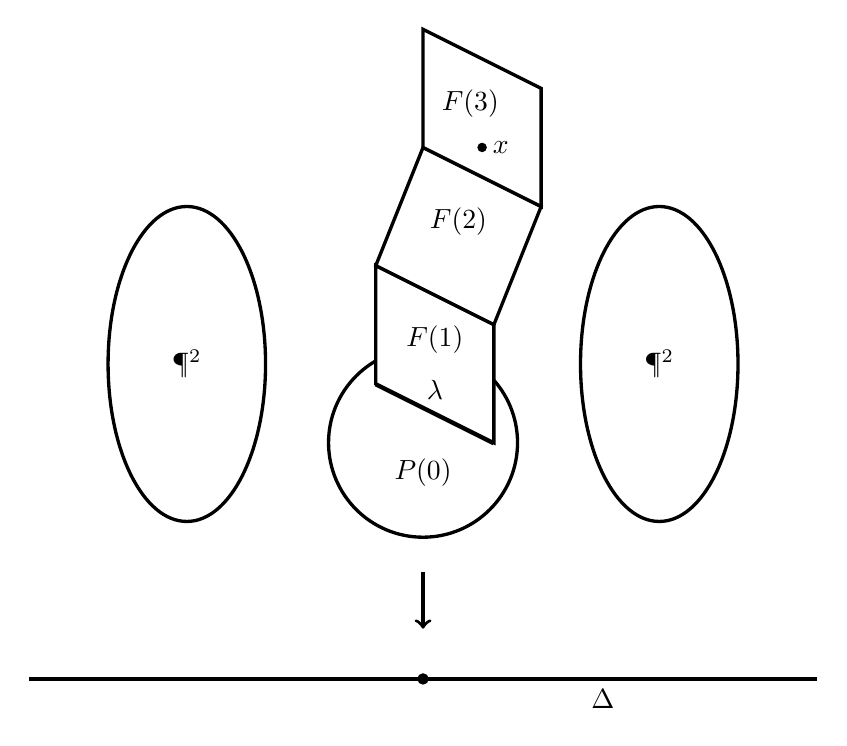
\begin{tikzpicture}[very thick]
  \begin{scope}[xshift=-3cm]
    \draw (0,0) ellipse (1 and 2);
    \draw (0,0) node {$\P^2$};
  \end{scope}
  \begin{scope}[yshift=-1cm, yscale=0.75, xscale=1.5]
    \draw(0,0) ellipse (0.8 and 1.6);
    \draw[line width=2] (-0.4,1) -- (0.6,0);
    \draw[fill=white] (-0.4,1) -- (0.6,0) -- (0.6, 2) -- (-0.4,3) -- cycle;
    \draw[fill=white] (0.6, 2) -- (-0.4,3) -- (0, 5) -- (1,4) -- cycle;
    \draw[fill=white] (0, 5) -- (1,4) -- (1,6) -- (0,7) -- cycle;
    \draw
    (0,-0.5) node {$P(0)$}
    (0.1,1.75) node {$F(1)$}
    (0.3, 3.75) node {$F(2)$}
    (0.4, 5.75) node {$F(3)$}
    (0.1, 0.9) node {$\lambda$};
    \draw[fill] (0.5, 5) ellipse (0.025 and 0.05) node [right] {$x$};
    \draw (0,-2) node (X) {};
  \end{scope}
  \begin{scope}[xshift=+3cm]
    \draw (0,0) ellipse (1 and 2);
    \draw (0,0) node {$\P^2$};
  \end{scope}
  \begin{scope}[yshift = -4cm]
    \draw (-5,0) -- (5,0) (2,0) node [below right] {$\Delta$};
    \draw[fill] (0,0) circle (0.05);
    \draw (0,0.5) node (D) {};
  \end{scope}
  \path  (X) edge [->] (D);
\end{tikzpicture}
%%% Local Variables:
%%% mode: latex
%%% TeX-master: "../main"
%%% End:
